\chapter{Proofs of UNSAT}
\label{sec:proofs}
\section{Introduction}

Neural network verifiers, like any other software, are prone to implementation bugs and unpredictable behavior on edge cases, which can be exploited~\cite{jia2021exploiting}. This phenomenon undermines the purpose of the verification process, and calls for mechanisms that ensure the reliability of verifiers.
A common practice for addressing solver reliability is the generation of \emph{proofs}: checkable mathematical objects that accompany verification results and serve as witnesses to their correctness. For satisfiable queries, correctness can be witnessed directly by a satisfying assignment. The unsatisfiable case, however, is more challenging to justify.

This chapter describes a standard format for expressing proofs of unsatisfiability for \vnnlib{} queries described in Section~\ref{sec:specification_language}.
A proof is intended to be written in a dedicated file written by the solver, which accompanies the \vnnlib{} specification and the ONNX network(s) files.
The goal is to modularly separate verifiers from proof checkers, enabling easier comparison between verifiers and checkers, and fostering the independent development of both.

The proof format is based on a subset of the Alethe proof format for SMT solving~\cite{ScFlBaFo21}. Alethe is a readable, resolution-based format for expressing the incremental derivation of first-order clauses from the input problem and previously derived clauses, using predefined \emph{proof rules}. The proof terminates with the derivation of the empty clause. One of the advantages of Alethe is that it allows solvers to leave \emph{proof holes} by invoking a dedicated rule, giving solvers flexibility in the level of detail included in the proof.
Another advantage is that Alethe proofs can be reconstructed as proof terms in several interactive theorem provers (ITPs)~\cite{LaFlBaJaAnReScBaTi25,EkMeTiKeKaReBa17,CoAnBaDoMe24}, and can also be checked by a capable standard proof checker~\cite{AnLaBa23}. Thus, using Alethe enables the reuse of existing state-of-the-art proof checkers.

\section{Proof Syntax}
\label{sec:proof-syntax}

\begin{figure}[p]
	\setlength{\grammarindent}{6.5em}
	\vspace{-0.8cm}
	\begin{grammar}\footnotesize
	<proof> ::=  <version><proofCommand>$^*$ 
	
	<proofCommand> ::= <assumeNetwork>
	\alt <assume>
	\alt<step>
	
	%<name> ::= [A-Za-z][\_A-Za-z0-9]*
	<assumeNetwork> ::=  (\texttt{assume-network} <name> <assumeNode>$^*$)
	
	<assumeNode> ::=  (\texttt{assume-node} <name> <nodeType> <assume>$^*$)
	
	
	<assume> ::= (\texttt{assume} <name> <bool>)

	<subproof> ::= (\texttt{anchor} :step <name>)
	
	<step> ::= (\texttt{step} <name> <clause> \texttt{:rule} <ruleName> <premisesAnnotation>$^?$ <argsAnnotation>$^?$ )
	
	<clause> ::= (\texttt{cl} <bool>$^*$)
	
	<premisesAnnotation> ::= \texttt{:premises} (<name>$^+$)
	
	<argsAnnotation> ::= \texttt{:args} (<rational>$^+$)
	
	<rational> ::= -$^?$[0-9]$^+$/$^?$[0-9]$^+$ 
	\alt -$^?$[0-9]$^+$(.[0-9]$^+$)$^?$
		
	<bool> ::= (\texttt{and} <bool> <bool>$^+$)
	\alt (\texttt{or} <bool> <bool>$^+$)
	\alt (\texttt{not} <bool>)
	\alt (\texttt{ite} <bool> <bool> <bool>)
	\alt (\texttt{\textless} <arith> <arith>)
	\alt (\texttt{\textless=} <arith> <arith>)
	\alt (\texttt{\textgreater} <arith> <arith>)
	\alt (\texttt{\textgreater=} <arith> <arith>)
	\alt (\texttt{==} <arith> <arith>)
	\alt (\texttt{!=} <arith> <arith>)
	\alt (\texttt{is\_int} <arith>)
	
	<ruleName> ::= \texttt{false} $\mid$ \texttt{not\_not}	
	\alt \texttt{resolution}
	\alt \texttt{or} $\mid$ \texttt{and\_pos} $\mid$ \texttt{and\_neg}
	\alt \texttt{ite1} $\mid$ \texttt{ite2}
	\alt \texttt{la\_totality} $\mid$ \texttt{la\_tautology} $\mid$ \texttt{la\_generic}
	\alt \texttt{bounded\_farkas} $\mid$ \texttt{hole}
	
	<nodeType> ::= \texttt{abs} $\mid$ \texttt{ceil} $\mid$ \texttt{clip} 
	\alt \texttt{floor} $\mid$ \texttt{gemm} $\mid$ \texttt{leaky\_relu}
	\alt \texttt{matmul} $\mid$ \texttt{max} $\mid$ 
	\alt \texttt{min} $\mid$ \texttt{relu} $\mid$ \texttt{sign}
	
	%<arith> ::= <element>$\networkTheoryVarParam$
	%\alt <name> <indices>$^?$
	%\alt (\texttt{-} <arith>)
	%\alt (\texttt{+} <arith> <arith>$^+$)
	%\alt (\texttt{*} <arith> <arith>$^+$)
	%\alt (\texttt{-} <arith> <arith>$^+$)
	
	%<indices> ::= [i, ..., i] for $i \in \mathbb{N}$
\end{grammar}
	\vspace{-1em}
    \caption{The syntax of \vnnlib{} proofs, adapted from the Alethe syntax in~\cite{ScFlBaFo21}, simplified and stylized for this context. The superscripts $^*$, $^+$, $^?$ and the terms <arith>,<name> and <version> are defined as in Figure~\ref{fig:vnnlib-syntax}.}
    \label{fig:proof-syntax}
\end{figure}

The syntax of \vnnlib{} proofs is shown in Figure~\ref{fig:proof-syntax}. At the top level, a \vnnlib{} proof consists of three parts:
\begin{enumerate}
	\item \textbf{Network assumptions:} Introduce formulas assumed to be correct by the structure of the neural networks. To ease proof checking, \vnnlib{} proofs specify the source of each network assumption depending on the context of their appearance:

	\begin{itemize}	
	\item The \texttt{assume-network} command specifies a \emph{network assumption context}. This command must name a network used in the \vnnlib{} specification file and it defines that network's context. This context is then used to define additional assumptions, imported from the declared network.
	\item Within a network context, the \texttt{assume} command specifies a constraint imported from that neural network. Each such assumption  must explicitly state the name of the ONNX layer used for its import, by using the \texttt{:layer} keyword. 
	\end{itemize}
	
	\item \textbf{Query assumptions:} Introduce formulas imported directly from the \vnnlib{} query specification, outside any network context. These assumptions are also introduced using the \texttt{assume} command and must reproduce formulas exactly as stated in the specification. Since they are defined outside any network context, they should not use the \texttt{:layer} keyword.

	All assumptions contain a unique identifier name and the imported formula. Additionally, the requirement to list the importing layer requires all ONNX networks used in this format to contain a unique name for each layer.
	For all assumptions declared outside an \texttt{assume-network} command, the \texttt{:layer} flag should lead to a checking failure.
	
	The proof checker \emph{must} certify that all network assumptions are correctly imported from a valid layer in the network, and that the variable names are consistent across all assumptions and with the ONNX files. All query assumptions must match an assertion defined in the \vnnlib{} specification file, and have consistent variable names with the other assumptions.
	
	\item \textbf{Proof steps:} Derive new facts from assumptions and from previously derived steps, called \emph{premises}. Each proof step contains a unique identifier name, the derived clause, the name of the proof rule used to derive it, its premises, and, when needed, additional rule-specific arguments.
	
	Proof steps may include \textbf{Subproofs}, which open a separate branch within a proof and add assumptions $A_1 \cdots A_n$. When concluding a subproof with a conclusion $C$, then clause $\lnot A_1, \dots, \lnot A_n, C$ is learned in the main proof branch.
\end{enumerate}
For simplicity, all assumptions must appear either: 
\begin{inparaenum}[(i)]
	\item before all proof steps to represent imported problem constraints; or
	\item immediately after beginning a subproof, to represent its local assumptions.
\end{inparaenum}

An example of a network, a specification defined in \vnnlib{}, and a corresponding Alethe proof appears at the end of this chapter in Section~\ref{sec:proof-example}.


\paragraph{Naming.} Formulas used in the proof can also be \emph{named} by a unique identifier, mainly for compactness and readability. Naming has the following syntax:

\begin{code}[style=lbnf]
	... !(term):named id ...
\end{code}


\paragraph{Variable Naming.} Although \vnnlib{} supported square brackets (\texttt{[ ]}) and commas (\texttt{,}) as a part of variable naming, Alethe does not. Therefore. to maintain the required consistency of variable names, we use underscores (\texttt{\_}) for indexing instead. For example, the variable $X[i,j]$ is indexed as $X\_i\_j$.

\subsection{Network Assumptions}
\label{sec:proof-assumptions}

We list the formal encodings of common ONNX nodes, including nodes frequently used in the neural network verification literature. We first formalize a general linear equation, which is used to encode linear nodes, and then present an alphabetical list of ONNX nodes together with their corresponding encodings.
For simplicity, we use a naming convention in which the input and output variables of each node are denoted by $x$ and $y$, respectively; and input and output matrices are denoted $A,B,C$ and $Y$, respectively. All node indexing that appear in the proofs must match the indexing implied by the node, and all variable naming must be isomorphic to such indexing.  

The list is not exhaustive, and we welcome contributions of encodings for additional node types.
 
\subsubsection{Linear Equations}

Linear equations are typically used to encode the affine transformations induced by the internal linear layers of the network, as well as linear constraints originating from the specification.
A linear equation of the form $d = \overset{l}{\underset{i=1}{\sum}} c_i \cdot x_i$  is represented in the proof
as: 

\begin{code}[style=lbnf]
(assume e (= d (+ (* c1 x1) ... (* ck xk))) :layer ...)
\end{code}

In particular, consider a linear equation that computes the value of a neuron from the values of neurons in a preceding layer. Let $X_k$ be a layer and $i_k$ be an index vector such that $X_k[i_k]$ denotes a neuron in that layer. Similarly, consider $m$ neurons from a preceding layer $X_j$, identified by the index vectors $i_1,\dots,i_m$, namely
$X_j[i_1],\dots,X_j[i_m]$.
Then, the computation: 
\[X_k[i_k] = c_1 \cdot X_j[i_1] + \cdots + c_m \cdot X_j[i_m] + b\] can be written as the assumption:

\begin{code}[style=lbnf]
(assume e (= Xk_ik (+ (* c1 Xj_i1) ... (* cm Xj_im) b))     :layer ...)
\end{code}


\subsubsection{ONNX Nodes Encoding}

\paragraph{Abs}
The constraint $y = \mathrm{abs}(x)$ is formulated as
follows: 

\begin{code}[style=lbnf]
(assume abs (ite (>= x 0.0) 
                   (= y x) 
                   (= y (- x))) :layer ...) 
\end{code}

\paragraph{Ceil}
This constraint requires introducing reasoning on integers (e.g. using reasoning over LIA). To this end, a constraint of the form 
$f = \mathrm{ceil}(x)$ is formulated as
follows: 

\begin{code}[style=lbnf]
(assume is_int y :layer ...)
(assume (< x (+ x 1)) :layer ...)
(assume (>= y x) :layer ...)
\end{code} 

where \texttt{is\_int} is the $LIA$ typecheck operator that returns true if and only if the type of its argument is \inlinevnn{int}. 


\paragraph{Clip}
The constraint $y = \mathrm{clip}_{M,m}(x)$, with maximum parameter $M$ and minimum parameter $m$ is formulated as
follows: 

\begin{code}[style=lbnf]
(assume clp1 (ite (>= x M) 
                    (= y M) 
                    (= y x)) :layer ...) 
(assume clp2 (ite (<= x m) 
                    (= y m) 
                    (= y x)) :layer ...) 
\end{code}

\paragraph{Floor}
This constraint requires introducing reasoning on integers (e.g. using reasoning over LIA). To this end, a constraint of the form 
And $y = \mathrm{floor}(x)$ is formulated as
follows: 

\begin{code}[style=lbnf]
(assume is_int y :layer ...)
(assume (> y (- x 1)) :layer ...)
(assume (<= y x) :layer ...)
\end{code} 

where \texttt{is\_int} is the $LIA$ typecheck operator that returns true if and only if the type of its argument is \inlinevnn{int}. 

\paragraph{Gemm (General Matrix Multiplication)}
The ONNX \texttt{Gemm} operator performs a general matrix multiplication followed by an addition. As input, the function receives three Tensors $A$, $B$, and $C$; two scalars $\alpha, \beta$; and two Booleans \texttt{transA}, \texttt{transB}. The operator computes
\[
Y = \alpha \cdot A'\cdot B' + \beta \cdot C,
\]

where $A'=A^\top$ if the \texttt{transA} attribute is set, and $A'=A$ otherwise; $B'$ is defined analogously according to \texttt{transB}. 
Assuming that $A'$ has dimensions $m\times k$ and $B'$
has dimensions $k\times n$, the resulting tensor $Y$ has dimensions $m\times n$, while $C$ is broadcast to $m\times n$ when necessary

To represent a fully connected layer, $B$ and $C$ are constant Tensors, resulting in
linear equations over the network variables of $A$.

Using the above formulation, we can assume the following equations used to derive the output variable $Y[i,j]$:
 
\begin{code}[style=lbnf,mathescape=true]
(assume e_i_j (= Y_i_j (+ (* $\alpha$ B_1_j A_i_1) ... 
                          (* $\alpha$ B_k_j A_i_k)
                          (* $\beta$ C_i_j))) :layer ...)
\end{code}

where \texttt{B\_1\_j,...,B\_k\_j, C\_i\_j } appear in their numerical value.


\paragraph{LeakyReLU}
The constraint $y = \mathrm{LeakyReLU}_\alpha(x)$, with leakage parameter $a>0$ is formulated as
follows: 

\begin{code}[style=lbnf]
(assume lr (ite (>= y 0.0) 
                  (= y x) 
                  (= y (* a x))) :layer ...) 
\end{code}

\paragraph{MatMul (Matrix Multiplication)}
The ONNX \texttt{MatMul} operator performs matrix multiplication. As input, the function receives two Tensors $A$ and $B$, and computes $Y = A \cdot B$.

For Tensors with more than two dimensions, the last two dimensions are treated as the matrix dimensions, while the preceding dimensions are treated as batch dimensions. Thus, considering a batch index vector $q$, and assuming that the last two dimensions of $A$ and $B$ are $m \times k$ and $k \times n$, respectively, each output variable is computed as:
\[
Y[q,i,j] = \sum_{r=1}^{k} A[q,i,r] \cdot B[q,r,j],
\]

To represent a linear layer, $B$ is a constant Tensor, resulting in linear equations over the network variables of $A$.
Using the above formulation, we can assume the following equations used to derive the output variable $Y[q,i,j]$:

\begin{code}[style=lbnf]
(assume e_q_i_j (= Y_q_i_j (+ (* B_q_1_j A_q_i_1) ... 
                              (* B_q_k_j A_q_i_k))) :layer ...)
\end{code}

where \texttt{B\_q\_1\_j,...,B\_q\_k\_j} appear in their numerical value.


\paragraph{Max and Min}
The constraint $y = \mathrm{max}(x_1,x_2)$ is formulated as follows: 
 
\begin{code}[style=lbnf]
(assume max (ite (>= x1 x2) 
                   (= y x1) 
                   (= y x2)) :layer ...) 
\end{code}

Likewise, $y = \mathrm{min}(x_1,x_2)$ is formulated as follows: 

\begin{code}[style=lbnf]
(assume min (ite (<= x1 x2) 
                   (= y x1) 
                   (= y x2)) :layer ...) 
\end{code}

Extending this formalization to multivariate  maximization and minimization is done by composition of the above formulation, i.e., by stating $max(a,b,c) = max(max(a,b),c))$.

\paragraph{ReLU} The constraint $y = \mathrm{ReLU}(x)$ is formulated as
follows: 

\begin{code}[style=lbnf]
(assume r (ite (>= x 0.0) 
                 (= y x) 
                 (<= y 0.0)) :layer ...) 
\end{code}

With the bound:

\begin{code}[style=lbnf]
(assume fl (>= y 0.0) :layer ...)
\end{code}

\paragraph{Sign}
The constraint $y = \mathrm{sign}(x)$ is formulated as
follows: 

\begin{code}[style=lbnf]
(assume sgn (ite (> x 0.0)
                 (= y 1.0)
                 (ite (< x 0.0)
                      (= y -1.0)
                      (= y 0.0))) :layer ...)
\end{code}

\subsection{Query Assumptions}

The syntactical form of query assumptions is independent of the neural network structure, and only adhere to constraints appear in the \vnnlib{} query file. In particular, variable naming in the proof file should be consistent with the naming in the query file.

For example, the notations above allows us to formalize any bounds on the form $l_j \leq X_j[i_j] \leq u_j$ for $l_j,u_j \in \mathbb{R}$ as:

\begin{code}[style=lbnf]
	(assert (>= Xj_ij lj))
	(assert (<= Xj_ij uj))
\end{code}

within the \vnnlib{} query. And as,

\begin{code}[style=lbnf]
	(assume l (>= Xj_ij lj))
	(assume u (<= Xj_ij uj))
\end{code}

within the proof file.

\subsection{Proof Steps}
 
\paragraph{Structure}
Recall that in Alethe, a proof step has the following form:

\noindent\begin{tabularx}{\linewidth}{ l C r }
		$s.\triangleright$ & 
		$\varphi_1,\dots,\varphi_n$ & 
		${\mathtt{(rule\_name \: s_1\cdots s_k)}[a_1 \cdots a_m]}$
\end{tabularx}\\
Where $\triangleright$ serves as a separator, $s$ is the unique step identifier, $\varphi_1 \cdots\varphi_n$ are terms representing a component of the derived clause, $\mathtt{s_1 \cdots s_k}$ are the identifiers of previous steps and assumptions, and  $\mathtt{a_1 \cdots a_m}$ are arguments with a specific definition per rule.

This general step is written as:

\begin{code}[style=lbnf,escapechar=@]
	(step s cl (@$\varphi_1 \cdots\varphi_n$@) :rule <rule_name> :premises(@$\mathtt{s_1 \cdots s_k}$@)
	                                      :args(@$\mathtt{a_1 \cdots a_m}$@))
\end{code}

We list here the subset of the Alethe proof rules that are used in the
\vnnlib{} proof format. Their complete description originally appears
in~\cite{ScFlBaFo21} and it is summarized here for completeness.

\paragraph{\texttt{false}:} A trivial rule introducing the negation of $\bot$.

\noindent\begin{tabularx}{\linewidth}{ l C r }
	$s.\triangleright$ & 
	$\lnot \bot$ & 
	${\mathtt{false}}$
\end{tabularx}

\paragraph{\texttt{not\_not}:} Enabling elimination of double negation.

\noindent\begin{tabularx}{\linewidth}{ l C r }
	$s.\triangleright$ & 
	$\lnot(\lnot\lnot\varphi),\varphi$ & 
	${\mathtt{not\_not}}$
\end{tabularx}

\paragraph{\texttt{resolution}:} This rules applies Boolean resolution, and can be applied for multiple premises at once.

\noindent\begin{tabularx}{\linewidth}{ l C r }
	$s.\triangleright$ & 
	$\varphi_1,\dots,\varphi_n$ & 
	${\mathtt{(resolution \: s_1\cdots s_k)}}$
\end{tabularx}

\paragraph{\texttt{or}:} The rule transform a disjunction of the form $\varphi_1\lor\cdots\lor\varphi_n$ to the clause $\mathtt{cl(\varphi_1 \: \cdots \: \varphi_n)}$.

\noindent\begin{tabularx}{\linewidth}{ l C r }
	$s.\triangleright$ & 
	$\varphi_1\lor\cdots\lor\varphi_n$ & 
	$(\cdots)$ \\
	
	$t.\triangleright$ &
	$\varphi_1,\dots,\varphi_n$ &
	${\mathtt{(or \: s)}}$
\end{tabularx}

\paragraph{\texttt{and\_pos} and \texttt{and\_neg}:} These two rules eliminate a conjunction or its negation.
A conjunction can be used to learn any one of its conjuncts, by using 
\texttt{and\_pos}:

\noindent\begin{tabularx}{\linewidth}{ l C r }
	$s.\triangleright$ & 
	$\lnot(\varphi_1\wedge\cdots\wedge\varphi_n),\varphi_k$ & 
	$\mathtt{and\_pos}[k]$
\end{tabularx}

Where $k\in[n]$.
Conversely, a from a sequence of formulas we can establish their conjunction, by using \texttt{and\_neg}:

\noindent\begin{tabularx}{\linewidth}{ l C r }
	$s.\triangleright$ & 
	$(\varphi_1\wedge\cdots\wedge\varphi_n),\lnot\varphi_1,\dots,\lnot\varphi_n$ & 
	$\mathtt{and\_neg}[k]$
\end{tabularx}

\paragraph{\texttt{ite1} and \texttt{ite2}:}
These two rules break an \texttt{ite} statement into clauses, alternating the truth value of the condition.


\noindent\begin{tabularx}{\linewidth}{ l C r }
	$s.\triangleright$ & 
	$\mathtt{ite \: \varphi_1 \: \varphi_2 \: \varphi_3}$ & 
	$(\cdots)$ \\
	$s1.\triangleright$ &
	$\lnot\varphi_1, \: \varphi_2$ &
	${\mathtt{(ite1 \: s)}}$ \\
	$s2.\triangleright$ &
	$\varphi_1, \: \varphi_3$ &
	${\mathtt{(ite2 \: s)}}$
\end{tabularx}

\paragraph{\texttt{la\textunderscore totality}:} This rule represents the order totality over the Reals. It is applied for \textsc{LRA} proof terms $t_1,t_2$.

\noindent\begin{tabularx}{\linewidth}{ l C r }
	$s.\triangleright$ & 
	$t_1\leq t_2 \: \lor \: t_2\leq t_1$ & 
	${\mathtt{(la\_totality)}}$
\end{tabularx}

\paragraph{\texttt{la\textunderscore tautology}:} This rule handles trivial cases for bounding a linear combination of variables $L_1$ with constants $d_1,d_2$. Generally, it has the form:

\noindent\begin{tabularx}{\linewidth}{ l C r }
	$s.\triangleright$ & 
	$\varphi_1 \: \lor \: \varphi_2$ & 
	${\mathtt{(la\_tautology)}}$
\end{tabularx} \\

For example, if $d_1=d_2$ we have that $L_1\geq d_1 \lor \lnot(L_1\geq d_2)$. The complete list of cases appears in~\cite{ScFlBaFo21}.

\paragraph{\texttt{la\textunderscore generic}:}
This rule is used to establish the unsatisfiability of a conjunction of linear atoms
$\psi_1 \wedge \cdots \wedge \psi_n$, and to derive the corresponding clause
$\mathtt{cl \: (\lnot\psi_1 \: \cdots \: \lnot\psi_n)}$.
The rule is parameterized by auxiliary arguments
$a_1,\ldots,a_n \in \mathbb{Q}$.

\noindent\begin{tabularx}{\linewidth}{ l C r }
	$s.\triangleright$ & 
	$\lnot\psi_1,\dots,\lnot\psi_n$ & 
	${\mathtt{(la\_generic)}[a_1 \: \cdots \: a_n]}$
\end{tabularx} \\

To check an application of the rule, each atom $\psi_i$ is first normalized, and the checker should compute a linear combination of the normalized atoms. The coefficient used for $\psi_i$ is $a_i$ when $\psi_i$ is an equality, and $|a_i|$ when $\psi_i$ is an inequality. The rule is valid if this linear combination simplifies to either $d \geq 0$ for some negative constant $d$, or to $d' > 0$ for some non-positive constant $d'$. In both cases, the resulting arithmetic contradiction certifies that the conjunction $\psi_1 \wedge \cdots \wedge \psi_n$ is unsatisfiable.
The complete checking procedure for this rule is given in~\cite{ScFlBaFo21}.



\paragraph{\texttt{hole}:} This rule indicates that the corresponding proof step has been left unproved by the verifier, and therefore marks a possible error or incompleteness in the proof.

\noindent\begin{tabularx}{\linewidth}{ l C r }
	$s.\triangleright$ & 
	$\varphi_1,\dots,\varphi_n$ & 
	${\mathtt{(hole \: s_1,\:\cdots\: s_k)}[a_1 \: \cdots \: a_m]}$
\end{tabularx} \\

A proof checker may either reject any proof containing such a step, or return a dedicated status indicating that all other proof steps are valid, while the proof as a whole remains incomplete.
The arguments and premises of this rule must be syntactically well formed, but they can be disregarded.
 
\paragraph{\texttt{bounded\textunderscore farkas}:}
In addition to the rules above, we include the option support the novel
\texttt{bounded\textunderscore farkas} rule, which formalizes the proof vectors
used in~\cite{IsBaZhKa22}. This rule provides a compact representation of
\texttt{la\textunderscore generic} for a particular class of cases, and can
therefore be reduced to an equivalent \texttt{la\textunderscore generic} step.

The rule derives the unsatisfiability of a sequence of linear equations
$\Theta_1,\ldots,\Theta_n$, followed by a sequence of simple linear inequalities
$\psi_1,\ldots,\psi_m$, where each inequality is of the form
$\psi_i := (x_i \bowtie c_i)$, with
$\bowtie \in \{<,>,\leq,\geq\}$, $c_i \in \mathbb{R}$, and $x_i$ a unique variable per inequality.
Using the above, the \texttt{bounded\textunderscore farkas} rule has the structure:

\noindent\begin{tabularx}{\linewidth}{ l C r }
	$s.\triangleright$ & 
	$\lnot\Theta_1,\dots,\lnot\Theta_n,\lnot\psi_1\cdots\lnot\psi_m$ & 
	${\mathtt{(bounded\_farkas)}[a_1 \: \cdots \: a_n]}$
\end{tabularx} \\

Observe that, unlike \texttt{la\textunderscore generic}, only the equations are associated with auxiliary arguments. The checking procedure for this rule follows from the variant of Farkas' lemma proved in~\cite{IsBaZhKa22}.

First, the checker computes the linear combination
$\sum_{i=1}^{n} a_i \cdot \Theta_i$, which yields an equation involving the variables that appear in the inequalities, say
$\sum_{j=1}^{m} c_j \cdot x_j = c$,
where $c_j \in \mathbb{R}\setminus\{0\}$. Then, for each variable $x_j$, the checker selects the inequality $\psi_{j'}$ containing $x_j$ and assigns it the coefficient $|c_j|$. Finally, the checker computes the combined expression
\[
\sum_{i=1}^{n} a_i \cdot \Theta_i
+
\sum_{j=1}^{m} |c_j| \cdot \psi_{j'} .
\]
For valid auxiliary arguments and selected inequalities, this expression should reduce to either $d \geq 0$ for some negative constant $d$, or to $d' > 0$ for some non-positive constant $d'$, as in \texttt{la\textunderscore generic}. In both cases, the result is an arithmetic contradiction, certifying the unsatisfiability of the original conjunction.
An additional form of this rule is as follows:

\noindent\begin{tabularx}{\linewidth}{ l C r }
	$s.\triangleright$ & 
	$\tau,\lnot\Theta_1,\dots,\lnot\Theta_n,\lnot\psi_1\cdots\lnot\psi_m$ & 
	${\mathtt{(bounded\_farkas)}[b,a_1 \: \cdots \: a_n]}$
\end{tabularx} \\

This form applies when the clause also contains a single simple inequality $\tau$, which is added to the linear combination with coefficient $b \in \mathbb{R}$. The checking procedure is analogous to the first form of the rule: the checker computes the linear combination of the equations using the coefficients $a_1,\ldots,a_n$, adds the contribution of $\tau$ with coefficient $b$, and then maps the remaining simple inequalities to coefficients as before. The resulting combination must again reduce to an arithmetic contradiction of the form $d \geq 0$ for some negative constant $d$, or $d' > 0$ for some non-positive constant $d'$.

\subsection{Subproofs}
\label{sec:subproofs}
A subproof opens a separate branch within a proof and is typically used to derive implications of the form $\varphi \rightarrow \psi$. A full description of subproofs appears in~\cite{ScFlBaFo21}.

A subproof begins with a sequence of assumptions that are valid only within its local context. It is introduced by an \texttt{anchor} command, which marks the start of the branch and specifies the identifier of the concluding step. The anchor is followed by one or more assumptions. Illustratively, this looks as:

\begin{code}[style=lbnf,escapechar=@]
	(anchor :step s)
	(assume a A)
\end{code}


The subproof is closed by a step using the \texttt{subproof} rule, which derives a conclusion clause of the form $\lnot\varphi_1,\ldots,\lnot\varphi_n,\psi$. At this point, the assumptions are said to be \emph{discharged}. Since the step applying the \texttt{subproof} rule terminates the subproof, its identifier must match the one specified in the corresponding \texttt{anchor}. The rule takes the concluding step $t$ of the subproof as a premise and explicitly lists the discharged assumptions.

\noindent\begin{tabularx}{\linewidth}{ l C r }
	$s_1.\triangleright$ &
	$\varphi_1$ &
	${\mathtt{assume}}$ \\
	
	& $\cdots$ & \\
	
	$s_n.\triangleright$ &
	$\varphi_n$ &
	${\mathtt{assume}}$ \\
	
	& $\cdots$ & \\
	
	$t.\triangleright$ &
	$\psi$ &
	${\mathtt{(...)}}$ \\


	$s.\triangleright$ & 
	$\lnot\varphi_1,\dots,\lnot\varphi_n,\psi$ & 
	${\mathtt{(subproof \: t)}[s_1 \: \cdots \: s_n]}$
\end{tabularx} \\

Therefore, concluding the above subproof anchor would have the form:

\begin{code}[style=lbnf,escapechar=@]
	...
	(step t (cl C ) :rule (...))
	(step s (cl (not A) C):rule subproof :premises(t)
                                      :discharge(a))
\end{code}

Nesting subproofs is possible, though if subproof $P$ is nested within $P'$, then $P$ must be completed before $P'$. 

\subsection{Comments and Whitespace}
Comments and Whitespace are used as in Section~\ref{sec:comments}.

\section{Example}
\label{sec:proof-example}
Lastly, this chapter is concluded with a complete example consisting of a neural network, a specification defined in \vnnlib{}, and a corresponding proof.

Consider the neural network and \vnnlib{} specification illustrated in Figure~\ref{fig:proof-query}. Assume that the matrix-multiplication layers defined by the ONNX file are as follows:

The input $X$ is multiplied by the matrix:

$$\begin{bmatrix} 1 & -1 & 0 
\\
0 & 1 & 1 
 \end{bmatrix}$$
resulting in: $$H = \begin{bmatrix} X\_0\_0 - X\_0\_1 
	\\
	X\_0\_1 + X\_0\_2
\end{bmatrix}$$.
The output of the hidden later $H$ is multiplied by the matrix:
$\begin{bmatrix} -1 & 1
\end{bmatrix}$. Meaning that $Y\_0\_0 = H\_0\_1 - H\_0\_0$.

Finally, assume that the input layer operator is named \texttt{il}, the hidden ReLU layer operator is named \texttt{hr}, and the output layer operator name is \texttt{ol}

\begin{figure}[h!]
	\begin{minipage}[c]{0.76\textwidth}
		\begin{lstlisting}[style=lbnf]   
			(declare-network encoder
			  (declare-input  X float64 [1,4])
			  (declare-hidden H float64 [1,2] "hr")
			  (declare-output Y float64 [1,1])
			)
			
			(assert (<= X_0_0 1.0))
			(assert (>= X_0_0 0.0))
			
			(assert (<= X_0_1 1.0))
			(assert (>= X_0_1 0.0))
			
			(assert (<= X_0_2 1.0))
			(assert (>= X_0_2 0.0))
			
			(assert (<= X_0_3 1.0))
			(assert (>= X_0_3 0.0))
			
			(assert (<= Y_0_0 -1.0)) \end{lstlisting}
	\end{minipage}
	\begin{minipage}[c]{0.21\textwidth}
		\centering
		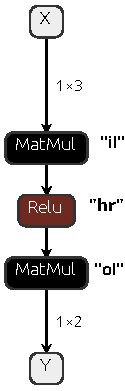
\includegraphics[height=6cm]{imgs/simple_encoder_net.onnx.pdf}
	\end{minipage}
	\caption{A \vnnlib{} network declaration that declares a hidden node}
	\label{fig:proof-query}
\end{figure}

An example proof of unsatisfiability for this query is shown in Figure~\ref{fig:proof}.
The proof introduces two variables for each hidden neuron in the ReLU layer \texttt{hidden}: \texttt{H\_0\_i\_b} and \texttt{H\_0\_i\_f} corresponding to the variables described in Section~\ref{sec:proof-syntax}.
The proof begins by declaring the network assumption in lines 2--14, which includes the equations induced by the linear layers of the network (lines 3--5), followed by assumptions encoding the ReLU activation constraints (lines 7--13). Then, in lines 17--23, the proof proceeds by importing bound assumption directly from the \vnnlib{} specification file.
Finally, lines 25--63 contain a sequence of derivation steps that lead to the empty clause, thereby establishing unsatisfiability.
\begin{figure}[p]
	\vspace{-0.8cm}
	\begin{lstlisting}[style=lbnf,basicstyle=\ttfamily\scriptsize\bfseries,linewidth=1.05\textwidth]
	; Network assumptions
	<@(assume network encoder @> 
	  (assume e1 (!(= (+ X_0_0 (- X_0_1 ) (- H_0_0_b)) 0.0):named e1) <@:layer@> il)
	  (assume e2 (!(= (+ (* 2.0 X_0_1) X_0_2 (- H_0_1_b)) 0.0):named e2) <@:layer@> il)
	  (assume e3 (!(= (+ H_0_1_f (- H_0_0_f) (- Y_0_0)) 0.0):named e3) <@:layer@> ol)
	
	  (assume r1 (!(ite (>= H_0_0_b 0.0)(= H_0_0_b H_0_0_f)(<= H_0_0_f 0.0)):named r1
	               )<@:layer@> hr)
	  (assume r2 (!(ite (>= H_0_1_b 0.0)(= H_0_1_b H_0_1_f)(<= H_0_1_f 0.0)):named r2
	               )<@:layer@> hr)
	
	  (assume lf0 (!(>= H_0_0_f 0.0):named lf0)<@:layer@> hr)
	  (assume lf1 (!(>= H_0_1_f 0.0):named lf1)<@:layer@> hr)
	<@)@>
	
	; Query assumption
	(assume u0 (!(<= X_0_0 1.0):named u0))
	(assume l0 (!(>= X_0_0 0.0):named l0))
	(assume u1 (!(<= X_0_1 1.0):named u1))
	(assume l1 (!(>= X_0_1 0.0):named l1))
	(assume u2 (!(<= X_0_2 1.0):named u2))
	(assume l2 (!(>= X_0_2 0.0):named l2))
	(assume u3 (!(<= Y_0_0 -2.0):named u3))
	
	; Prove for both ReLUs that f - b >= 0
	(step t1 (cl (not (>= H_0_0_b 0.0))(= H_0_0_b H_0_0_f)):rule ite2 :premises(r1))
	(step t2 (cl (not (= H_0_0_b H_0_0_f))(<= 0.0 (- H_0_0_f H_0_0_b))):rule
	         la_generic :args(-1 1))
	(step t3 (cl (>= H_0_0_b 0.0)(not (>= H_0_0_f 0.0))(<= 0.0 (- H_0_0_f H_0_0_b)))
	         :rule la_generic :args(1 -1 1))
	(step aux1bound (cl (<= 0.0 (!(- H_0_0_f H_0_0_b):named H_0_0_a))):rule
	                resolution :premises(t1 t2 t3 lf0))
	(step s1 (cl (not (>= H_0_1_b 0.0))(= H_0_1_b H_0_1_f)):rule ite2 :premises(r2))
	(step s2 (cl (not (= H_0_1_b H_0_1_f))(<= 0.0 (- H_0_1_f H_0_1_b))):rule 
	         la_generic :args(-1 1))
	(step s3 (cl (>= H_0_1_b 0.0)(not (>= H_0_1_f 0.0))(<= 0.0 (- H_0_1_f H_0_1_b))) 
	         :rule la_generic :args(1 -1 1))
	(step aux2bound (cl (<= 0.0 (!(- H_0_1_f H_0_1_b):named H_0_1_a))):rule 
	                resolution :premises(s1 s2 s3 lf1))
	                
	; Activation pattern reasoning
	(step ax1 (cl (>= H_0_0_b 0.0)(<= H_0_0_f 0.0)):rule ite1 :premises(r1))
	(step ax2 (cl (not (>= H_0_0_b 0.0))(= H_0_0_b H_0_0_f)):rule ite2 :premises(r1))
	(step ax3 (cl (not (= H_0_0_b H_0_0_f))(<= H_0_0_a 0.0)):rule la_generic 
	          :args(1 1))
	(step ax4 (cl (not (>= H_0_0_b 0.0))(<= H_0_0_a 0.0)):rule resolution 
	          :premises(ax2 ax3))
	
	; Prove UNSAT for both phases of H_0_0
	(step lf1 (cl (not e3)(not lf1)(not u3)(not (<= H_0_0_f 0.0))):rule la_generic 
	          :args(-1 1 1 1))
	(step lf2 (cl (not (<= H_0_0_f 0.0))):rule resolution :premises(lf1 e3 lf1 u3))
	(step lf3 (cl (>= H_0_0_b 0.0)):rule resolution :premises(ax1 lf2))
	
	(step rt1 (cl (not e1)(not e2)(not e3)(not l1)(not l2)(not u0)(not u3)
	          (not (<= H_0_0_a 0.0))(not (<= 0.0 H_0_1_a))):rule la_generic 
	          :args(1 -1 -1 3 1 1 1 -1 -1))
	(step rt2 (cl (not (<= H_0_0_a 0.0))):rule resolution 
	          :premises (rt1 e1 e2 e3 l1 l2 u0 u3 aux2bound))
	(step rt3 (cl (not (>= H_0_0_b 0.0))):rule resolution :premises(rt2 ax4))
	
	; Finalize
	(step final (cl):rule resolution :premises(rt3 lf3))\end{lstlisting}
	\vspace{-0.4cm}
	\caption{An example for a \vnnlib{} proof in Alethe. The text highlighted in red is an addition on top of the standard Alethe.}
	\label{fig:proof}
\end{figure}
